 \chapter{Methodology}\label{ch:methodology}

In this chapter, the test equipment and experiment procedures are presented. The experiment is based on the planetary test rig in UNSW. Vibration signals are collected by a National Instrument data acquisition system and analyzed in Matlab.

\section{Equipment}

The test equipment includes the planetary gearbox test rig, control system, and the data acquisition system.

\subsection{Planetary gearbox test rig}

The UNSW planetary gearbox test rig was firstly built by Sweeney in a parallel configuration and then modified to the planetary configuration. Seen from the layout in Figure 3.1, the test rig is driven by a 3 Phase AC induction motor and a hydraulic pump provided the resistance torque. Two flywheels are mounted on input and output shaft to minimize speed fluctuation.
Power is transferred through the planetary gearbox in the center. The planetary has a parallel stage and a planetary stage. The input of the parallel stage is a 42-tooth pinion gear, and the output is a 55-tooth spur gear fixed to the planet carrier. The planetary stage is driven by the planet carrier. It carries tree planet gears which have 23 teeth each. The ring is fixed and has 80 teeth. The output sun gear has 34 teeth.

\begin{figure}[h]
	\centering
	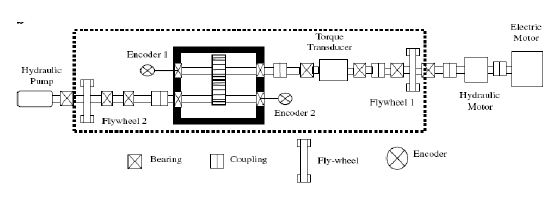
\includegraphics{rig}
	\caption{UNSW planetary gearbox test rig}
	\label{testrig}
\end{figure}

The gearbox is connected to the input and output shafts by belt couplings, which are not shown in the layout of Figure 3.1. The tension of the belts is adjusted by the sliding rails downside the gearbox housing. The planetary gearbox and the belt drives are illustrated in Figure 3.2.

An in-line torque transducer is used to measure the torque on the drive shaft. Its result is shown directly on The UNSW MK II transducer indicator. Due to the limitation of the belt transmission, the maximum torque is restricted to 70 Nm.
A Hidden 426-36000 shaft encoder is mounted on the input shaft of the gearbox. Which is shown in the upper-left corner of Figure 3.2. 
The external accelerometer is fixed by a stud to the outframe of the ring gear. There are two internal accelerometers, axial and radial, mounted inside the spur gear. The radial transducer rotates together with the carrier, and its signal is transferred out through a Michigan Scientific B6-2 slip ring on the left side. Both the external and internal transducers are Bruel \& Kjaer 4394 IEPE accelerometers.

\begin{figure}[h]
	\centering
	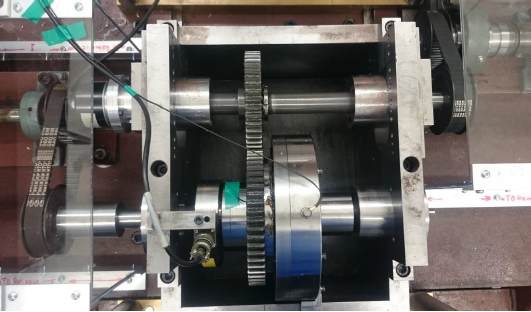
\includegraphics[scale = 0.7]{gearbox}
	\caption{The planetary gearbox}
	\label{gearbox}
\end{figure}

The speed of the AC induction motor is controlled by a FRENIC-MEGA variable frequency drive (VFD), which allows us to run the variable speed tests. As this is an 8 pole induction motor, the input frequency displayed on the variable frequency drive should be divided by four to get the drive shaft running frequency. The speed of the shaft could be controlled directly on the VFD using increase and decrease buttons or remotely controlled on the computer by the program. The VFD is what makes the variable speed test feasible.

The VFD is installed on the control panel together with its switch and an emergency stop button.  It also contains the hydraulic control valve and the hydraulic isolation valve. The resistance torque could be adjusted by the control valve. Two torque mode is provided: high torque and low torque. The control panel is shown in Figure 3.3.

\begin{figure}[h]
	\centering
	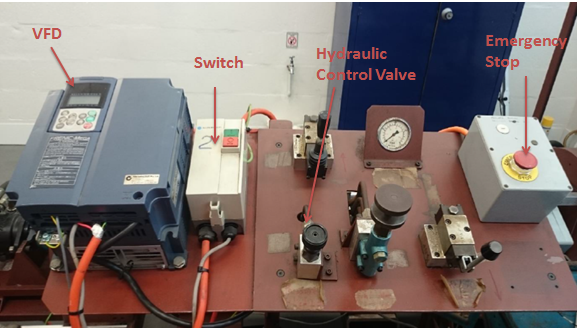
\includegraphics[scale = 0.7]{control}
	\caption{The control panel of the test rig}
	\label{control panel}
\end{figure}

\subsection{Data acquisition system}

The test signals generated by the rig are collected by a National Instrument (NI) PXI data acquisition system which is embedded with an internal PC. Data are collected and displayed through LabView. The collected data are finally processed in Matlab.

The PXIe-1071 system is an integrated data acquisition platform. It is widely used in machine monitoring, automotive and industrial test. The analog signal is conditioned and A/D converted by the data acquisition system and the digital signal is displayed and further processed in the computer. Chanel numbers of the PXI system is adjustable according to the chosen modules. It requires 2 vibration channel and one tacho channel to run this project.

\begin{figure}[h]
	\centering
	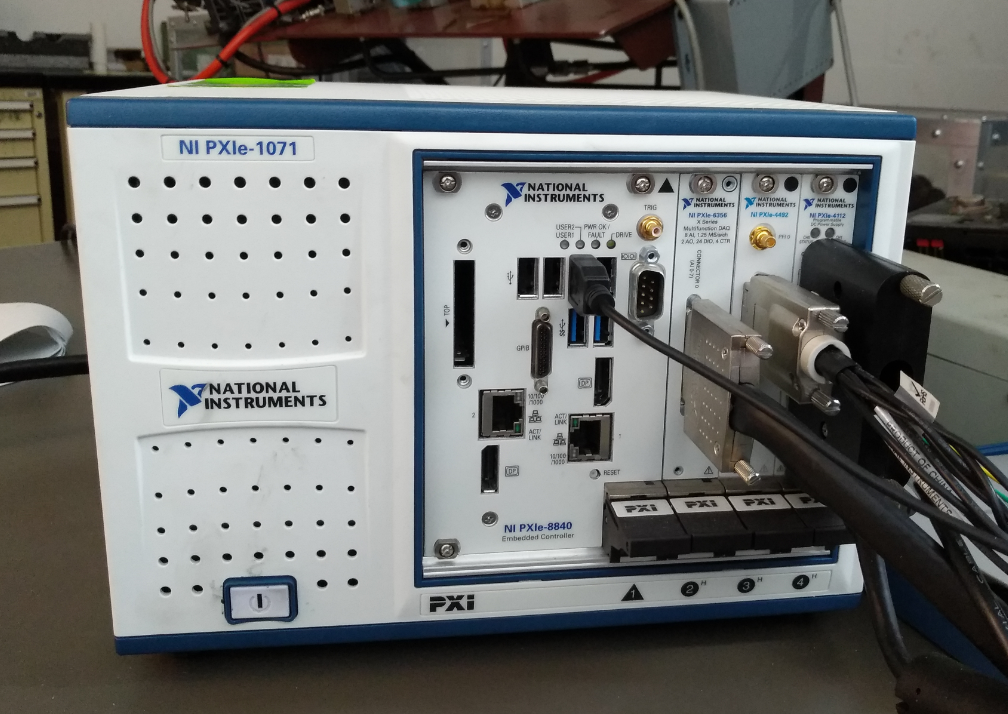
\includegraphics[scale = 0.4]{NI}
	\caption{The data acquisition system}
	\label{data acuisition}
\end{figure}

\section{Test Settings}

In this project, three test settings are conducted with the same gear fault. The first test is a speed up process in certain acceleration. The second test is a two-stage speed up process with different accelerations. The last is a speed fluctuation process. Comparisons are made to verify the developed diagnosis procedure.

\subsection{Test 1}

The first test is a run-up process. It starts at 1 Hz, which is 4 Hz on the variable frequency drive due to the 8-pole induction motor, and end at 6 Hz (24 Hz on VFD). The whole process takes 50 seconds and the shaft speed increase in a relatively constant acceleration. The load is set to be in low-loading mode. The speed profile is shown in the following figure. This test is to simulate the start-up process of the monitored machine. There could be a variety of incidents in the start-up stage, and a sooner detection of fault could prevent further damage effectively.

In this process, as the speed increases, the vibration amplitude increases accordingly. When it goes through resonance frequencies, even larger amplitude should be shown on its time domain waveform. This resonance could be compensated by performing of exponential liftering in theory.

\begin{figure}[h]
	\centering
	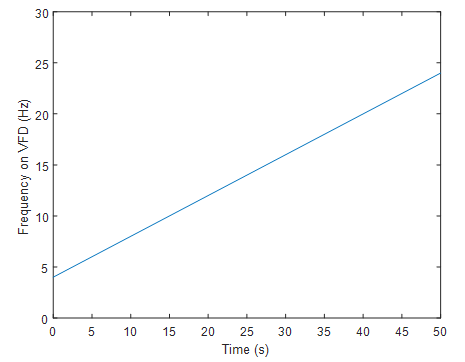
\includegraphics{speedup}
	\caption{Speed-up profile}
	\label{test1}
\end{figure}

\subsection{Test 2}

The speed profile of the second test is shown in Figure 3.6. It started from zero Hz and increased to 4 Hz (16 Hz on VFD) at a constant acceleration in 30 seconds. It stayed at this running speed for 20 seconds and went up to 6 Hz (24 Hz on VFD) in 30 seconds. The speed remained constant for another 20 seconds and then decreased to zero. This simulation is a whole process of the monitored machine from start-up to operation in different conditions and finally shut down.

During this test, seen from the speed profile, the accelerations are different in the two speed-up process and the slow-down process. The two constant speed platform would be analyzed as comparisons.

\begin{figure}[h]
	\centering
	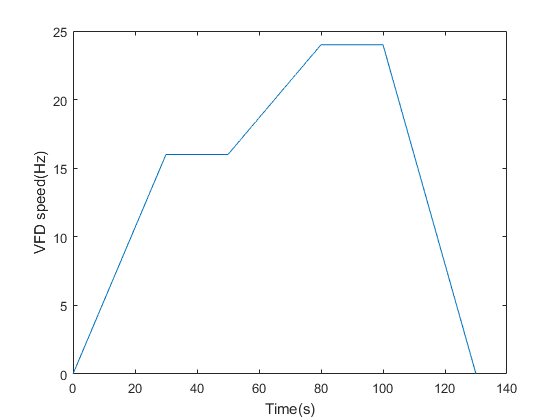
\includegraphics[scale = 0.85]{test2}
	\caption{Test 2 speed profile}
	\label{test2}
\end{figure}

\subsection{Test 3}

Many rotating machines such as automobile and wind generators operate in varying speed. Which brought challenges to the vibration based machine condition monitoring. In test 3, the varying speed process is simulated. The input shaft of the planetary gearbox was accelerated from zero to 5 Hz (20 Hz on VFD) in 30 seconds. Then it varies in a sinusoidal wave around 5 Hz for $\pm$25\%. After 4 cycles and 120 seconds, the machine was shut down to zero Hz. The speed profile of the whole process is shown below in Figure 3.7. This test is run on the low torque mode.

\begin{figure}[h]
	\centering
	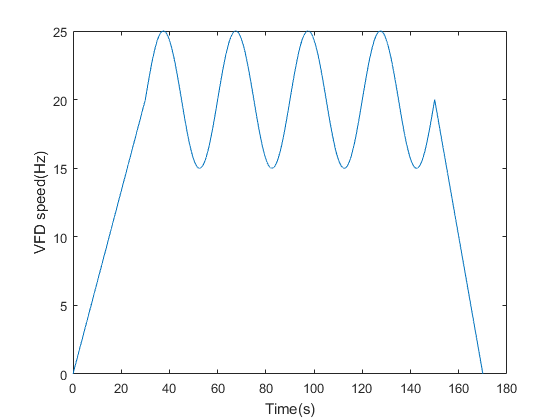
\includegraphics[scale = 0.85]{test3}
	\caption{Test 3 speed profile}
	\label{test3}
\end{figure}

\section{Processing and Analysis}

The data processing and analysis is extensively based on MATLAB. Data collected by NI PXI and LabView is stored in separate documents. It was first organized in MATLAB according to time and signal type. Each channel of the signal is stored as a vector. Additional messages such as torque and sample rate are supplied for further analysis. The investigated signal for our project is the external vibration and the tacho signal. The vibration signal holds the fault information of the gearbox, while the tacho gives running speed and phase information.

As discussed in chapter 2.4, the processing procedure is:

\begin{enumerate}
	\item Perform cepstrum modification for resonance compensation;
	
	\item Order tracking to avoid discrete frequency smearing due to the speed variation;
	
	\item Hilbert transform for demodulation.
	
\end{enumerate}

In this stage, only test 1 was performed, and all the processing and analysis is based on the data of test 1. The time domain vibration waveform from the external sensor is illustrated in Figure 3.8(1). As seen from the plot, the vibration amplitude increase according to the shaft speed. So the vibration signal is dominated by the largest last 10 seconds, which is shown in Figure 3.8(2).

\begin{figure}[htbp]
	\centering
	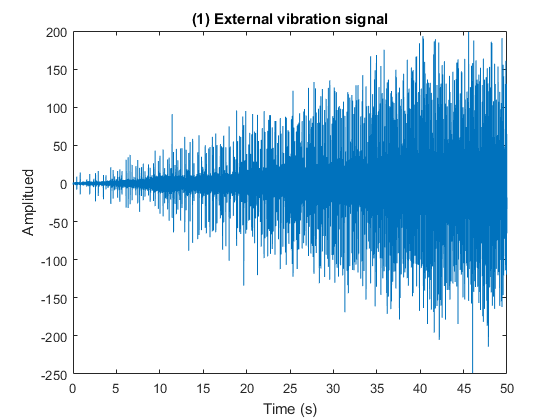
\includegraphics[scale =0.48]{wave}
	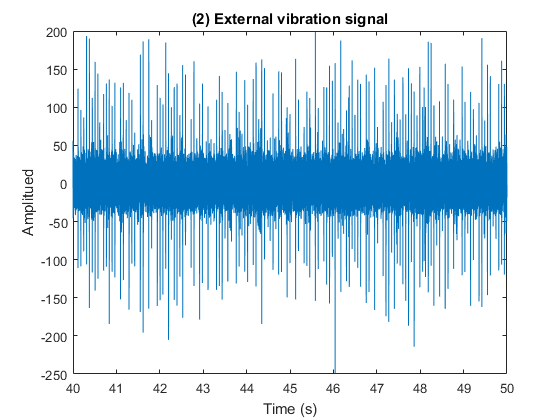
\includegraphics[scale =0.48]{last10}
	\caption{Vibration waveform of different period}
	\label{wave1}
\end{figure}

The first step, resonance compensation based on cepstrum modification, is performed on the signal of the whole period and that of the last 10 seconds. The liftered waveforms are shown as below:

\begin{figure}[h]
	\centering
	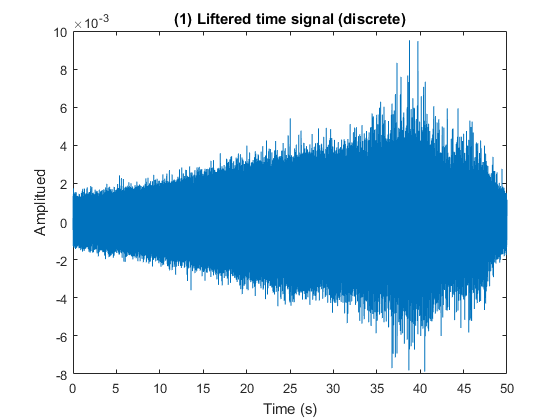
\includegraphics[scale =0.48]{wavelift}
	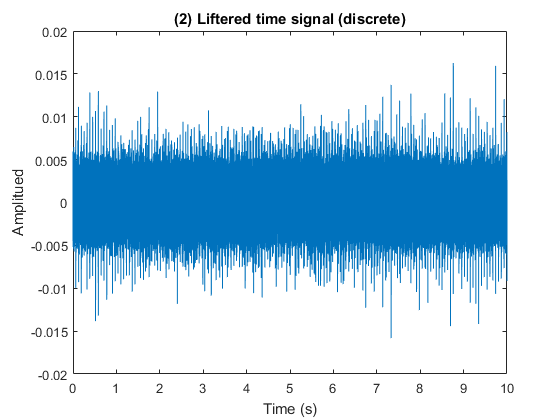
\includegraphics[scale =0.48]{last10lift}
	\caption{Liftered vibration waveform of different period}
	\label{wave2}
\end{figure}

Seen from Figure 3.8 and 3.9, the liftered signals are smaller and more uniform than the original ones. Looking into Figure 3.8 (1), it is able to be seen that there is an amplitude increase around 10 seconds. It could be the shaft passing through a resonance frequency. The liftered signal in Figure 3.9 (1), on the other hand, shows no other change besides the increasing along speed.

The second step is order tracking. This method is based on phase demodulation of the phase-locked tacho as a reference. A same number of samples are taken from each revolution. The order tracking method eliminates the effect of speed variation. When performing order tracking, the running speed is based on the tacho signal taken from the input shaft, and then transferred to carrier shaft speed by their gear ratio. Thus the carrier frequency is 1 Hz. Running frequency of other gears could be calculated based on it.

The last step is amplitude demodulation based on Hilbert transform. As discussed in the former part, the deterministic part of gear vibration is gear mesh signal. The shocks produced by gear fault are impulses in a lower frequency, which could be treated as amplitude modulation signal carried by the gear mesh frequency. In this condition, the Hilbert transform or envelope analysis is able to demodulate the faulty signal. At last, the spectrum of the amplitude information of the Hilbert transformed signal would reveal the faulty frequency. A comparison with each gear frequency would tell which one is with malfunction. 












